\begin{figure}[t]
\centering
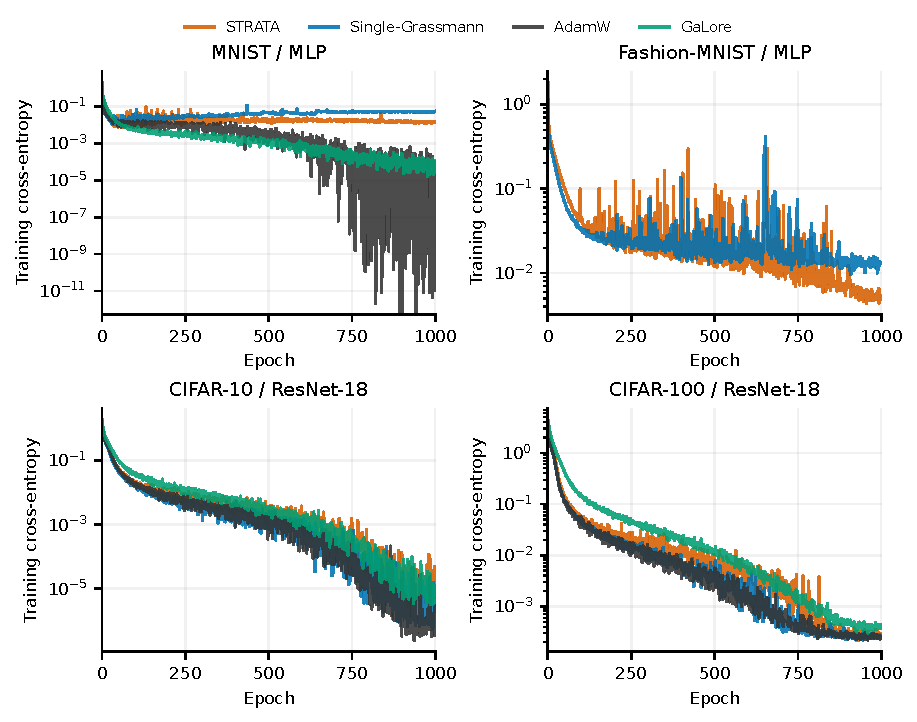
\includegraphics[width=\linewidth]{figures/fig_loss_classification.pdf}
\caption{\textbf{Full 1000-epoch training-loss trajectories.} Four archived classification settings, seed 42. Within each available method grid we select a completed run by terminal-100 validation accuracy and plot its raw training cross-entropy. Baseline grids have unequal sizes; these panels are descriptive convergence comparisons, not an equal-search causal experiment. No smoothing, extrapolation, seed averaging, or test-based selection is used. Training and validation curves for the same runs, every completed classifier-grid loss, fixed-rank PINN curves, graph/continual curves, and separately labeled ongoing runs appear in Appendix~\ref{app:loss-trajectories}.}
\label{fig:loss-classification}
\end{figure}
\paragraph{Loss trajectories and generalization.}
Figure~\ref{fig:loss-classification} replaces endpoint-only inspection with complete recorded optimization paths. Low training cross-entropy does not establish a test-accuracy advantage. The accompanying held-out cross-entropies expose late overfitting and confidence effects that accuracy alone can conceal. Appendix~\ref{app:loss-trajectories} retains both curves and adverse hyperparameter outcomes. All observed epochs are plotted; an archived index of zero is the first logged trained epoch, not a reconstructed common initialization.
